\subsubsection{Caso d'uso UC8.1.6: Creazione esercizio a riempimento di spazi vuoti}
	\label{UC8.1.6}
	\begin{figure}[h]
		\centering
			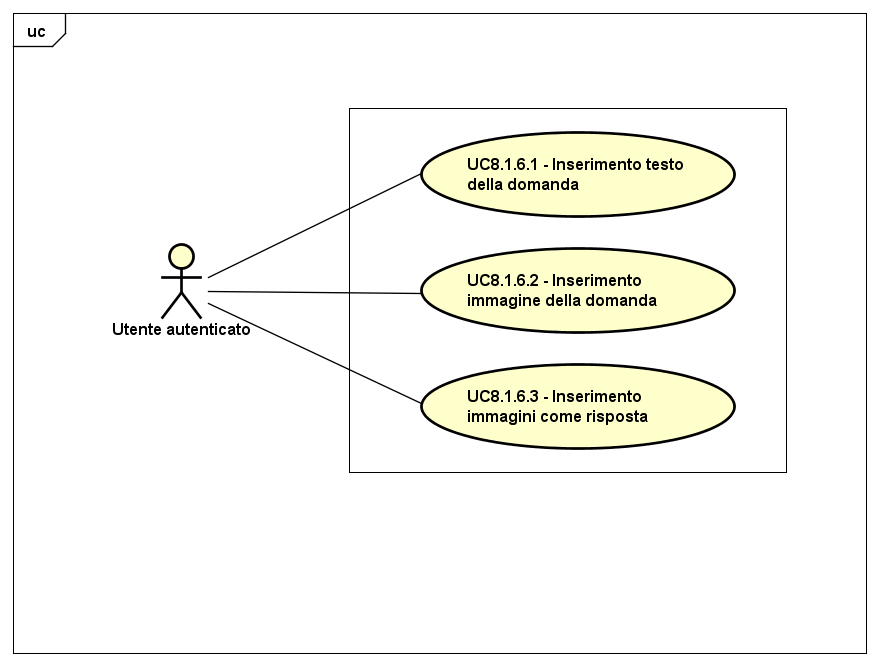
\includegraphics[scale=0.45,keepaspectratio]{UML/UC8_1_6.png}
		\caption{UC8.1.6: Creazione esercizio a riempimento di spazi vuoti}
	\end{figure}
	\FloatBarrier
	\begin{itemize}
		\item
			\textbf{Attori}: utente autenticato, utente autenticato pro;
		\item		
			\textbf{Descrizione}: l'attore può utilizzare la procedura guidata per la creazione di un esercizio a riempimento di spazi vuoti;
		\item
			\textbf{Precondizione}: il sistema presenta all'attore la procedura guidata per la creazione di un esercizio a riempimento di spazi vuoti;
		\item
			\textbf{Postcondizione}: l'attore ha creato un esercizio a riempimento di spazi vuoti;
		\item
			\textbf{Scenario principale}:
	       		\begin{enumerate}
	       			\item
	       			L'attore può inserire il testo dell'esercizio (UC8.1.6.1);
	       			\item
	       			L'attore può indicare le parole che saranno sostituite con degli spazi vuoti dal sistema (UC8.1.6.2).
	 			\end{enumerate}
	\end{itemize}
	
\subsubsection{Caso d'uso UC8.1.6.1: Scrittura testo dell'esercizio}
	\begin{itemize}
		\item
			\textbf{Attori}: utente autenticato, utente autenticato pro;
		\item		
			\textbf{Descrizione}: l'attore può inserire il testo dell'esercizio;
		\item
			\textbf{Precondizione}: il sistema presenta all'attore lo spazio destinato all'inserimento del testo dell'esercizio; 
		\item
			\textbf{Postcondizione}: l'attore ha scritto il testo dell'esercizio;
		\item
			\textbf{Scenario principale}: l'attore scrive il testo dell'esercizio.
	\end{itemize}


\subsubsection{Caso d'uso UC8.1.6.2: Indicazione parole da oscurare}
	\begin{itemize}
		\item
			\textbf{Attori}: utente autenticato, utente autenticato pro;
		\item		
			\textbf{Descrizione}: l'attore può indicare le parole che saranno sostituite con degli spazi vuoti;
		\item
			\textbf{Precondizione}: il sistema presenta all'attore lo spazio destinato all'indicazione delle parole da oscurare;  
		\item
			\textbf{Postcondizione}: l'attore ha indicato le parole che saranno sostituite con degli spazi vuoti;
		\item
			\textbf{Scenario principale}: l'attore indica le parole che verranno oscurate dal sistema.
	\end{itemize}